\documentclass[a4paper, 12pt]{report}

\usepackage{graphicx}
\usepackage{textcomp}
\usepackage[italian]{babel}
\usepackage[a4paper, total={17cm, 24cm}]{geometry}
\usepackage{float}
\usepackage[font=small,format=plain,labelfont=bf,up,textfont=normal,up,justification=justified,singlelinecheck=false,skip=0.01\linewidth]{caption}
\renewcommand{\familydefault}{\sfdefault}

\title{Relazione progetto\\``Smart Dumpster''}
\author{Matteo Castellucci, Giorgia Rondinini}
\date{\today}

\begin{document}
	\maketitle
	\tableofcontents
	\chapter{Analisi dei requisiti}
	Si vuole realizzare un sistema di deposito rifiuti intelligente denominato ``Smart Dumpster".\newline
	Questo sistema dovrà permettere all'utente il deposito dei rifiuti tramite un'\textit{app} Android
	previo l'ottenimento di un codice speciale denominato ``token" da un componente che esegue su un
	\textit{host} separato dal bidone fisico definito ``Service". Una volta ottenuto il token occorre
	recarsi nei pressi del bidone, e collegarsi tramite Bluetooth alla componente ``Controller" del
	sistema entro cinque minuti, pena la scadenza del token. Ad avvenuto collegamento, è
	possibile scegliere il tipo di rifiuto da depositare ed
	effettuare così richiesta per un deposito. L'app contatterà per primo il Service, notificandolo della
	richiesta e, se sarà possibile effettuarla - ovverosia il sistema è nello stato ``\textit{available}"
	e il token passato al Service è lo stesso fornito poco prima dal Service all'app -, esso procederà
	con il notificare a sua volta la componente ``Edge" del sistema. Se questa operazione va a buon fine, 
	si notifica il Controller di voler effettuare un deposito fornendo anche il tipo di rifiuto che si
	vuole depositare scegliendolo tra tre tipi - A, B o C - e questo aprirà gli sportelli per permettere
	all'utente di depositare i rifiuti. L'utente
	avrà trenta secondi per effettuare un deposito, dopo il quale le porte si chiuderanno e il bidone
	incamererà i rifiuti depositati. A questo punto, la componente Controller invierà un messaggio di
	terminazione deposito all'applicazione che a sua volta notificherà il Service. Nel caso in cui
	l'utente abbia inserito troppi rifiuti eccedendo il peso massimo che il bidone può contenere, la
	componente Edge si preoccuperà di notificare il Service, inviandogli anche il peso caricato fino a
	quel punto e questo si preoccuperà di impostare lo stato del sistema su ``unavailable". Se questo è
	il caso, il Service non si preoccuperà di notificare la terminazione del deposito anche all'Edge,
	essendo per lui già terminato. In caso contrario lo farà, ottenendo dall'Edge il peso dei rifiuti
	inseriti dall'utente.\newline
	Il sistema presenterà anche un sito web denominato ``Dashboard", di esclusivo accesso agli operatori
	ambientali, che permetterà di pilotare il Service,
	ovvero sarà possibile vedere se il sistema si trova nello stato ``\textit{available}" o
	``\textit{unavailable}", qual è il peso corrente dei rifiuti contenuti nel bidone e il numero di
	depositi giornalieri effettuati. Inoltre, sarà possibile richiedere separatamente il \textit{log},
	ovvero il numero di depositi e la quantità totale depositata negli ultimi cinque giorni. Sarà
	possibile anche forzare lo stato del sistema per ragioni di manutenzione a ``\textit{available}" o
	``\textit{not available}" in qualsiasi momento, anche durante un deposito, tenendo conto del fatto
	che forzare lo stato del bidone a ``available" significa anche averlo svuotato e perciò il peso
	correntemente contenuto al suo interno sarà azzerato.
	\begin{figure}[H]
		\centering
		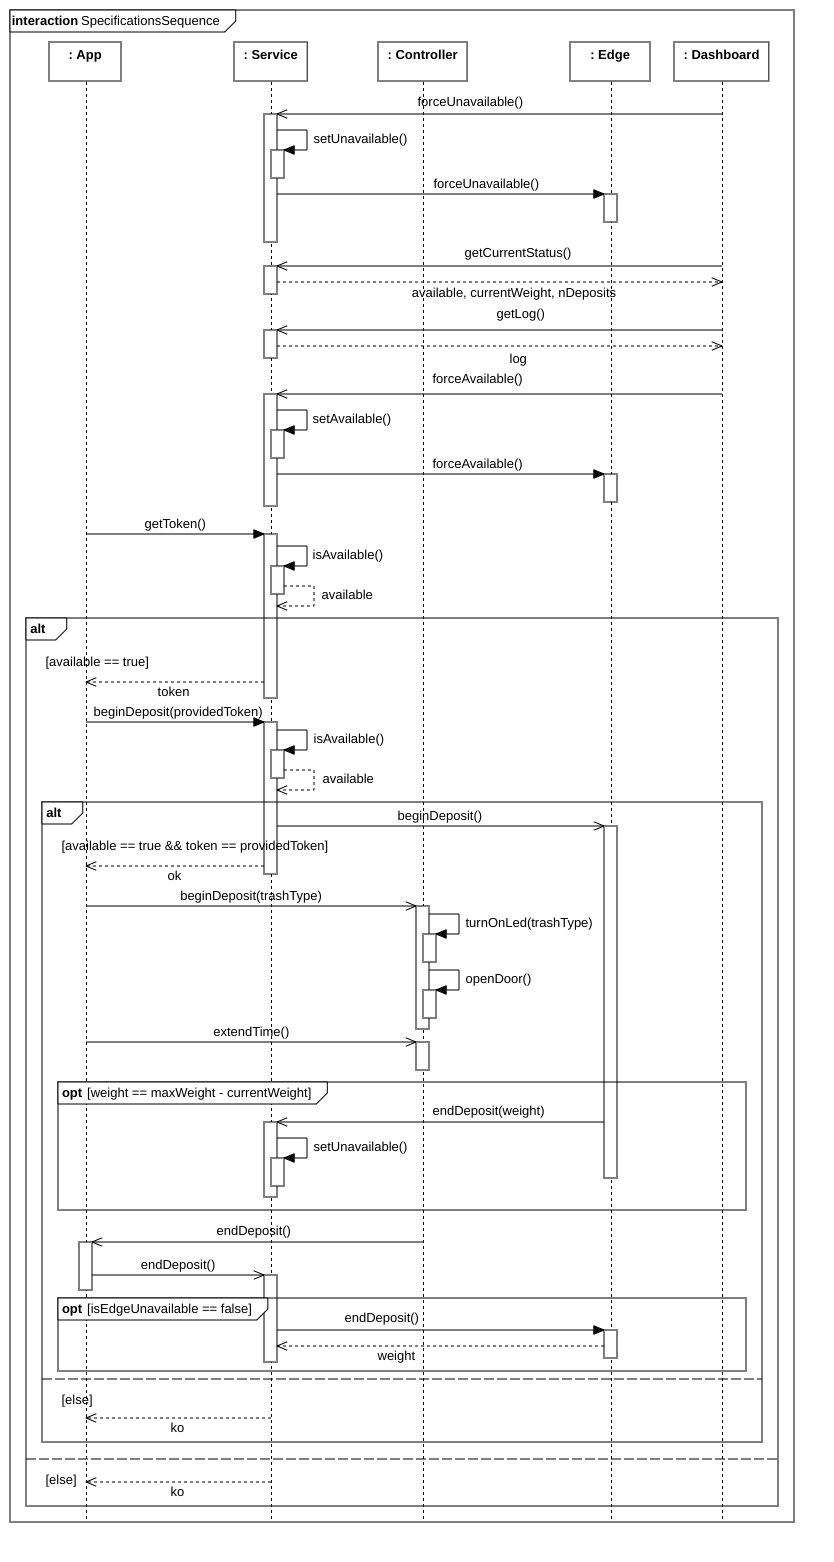
\includegraphics[height=\textheight]{"img/Sequence.png"}    
		\caption{Diagramma di sequenza con le interazioni tra le componenti del sistema}
	\end{figure}
	\begin{figure}[H]
		\centering
		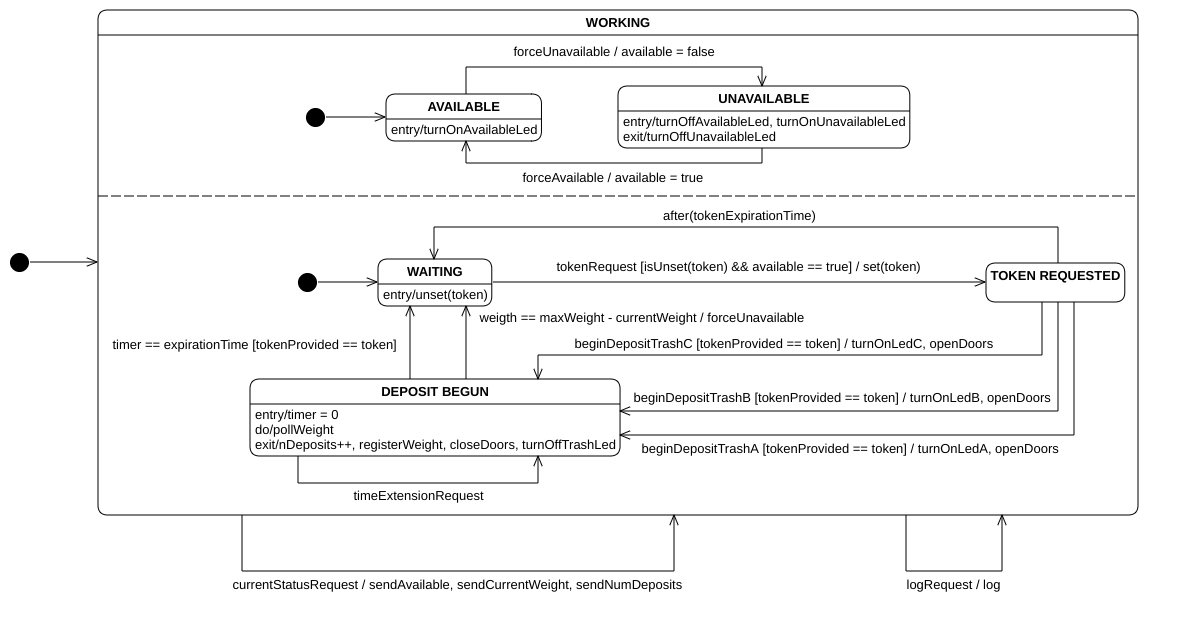
\includegraphics[width=\textwidth]{"img/SystemStatechart.png"}    
		\caption{Diagramma di stato del sistema nel suo complesso}
	\end{figure}
	\chapter{Design}
		\section{Specifiche hardware e schemi dei circuiti}
		Gli stati ``\textit{available}" e ``\textit{not available}" sono fisicamente rappresentati sul sistema da due LED,
		rispettivamente uno verde e uno rosso. Il sensore di peso utilizzato durante il deposito è
		rappresentato da un potenziometro e, assieme ai due LED, è pilotato alla componente Edge del
		sistema, realizzata su un SoC ESP8266 ``NodeMCU 1.0".\newline
		Ai tre tipi di rifiuti sono associati altrettanti LED verdi e prima del deposito viene acceso
		quello corrispondente al tipo di rifiuto scelto e non viene spento fino al termine dello stesso.
		L'apertura e la chiusura degli sportelli sono pilotate da un servomotore, che come i tre LED
		sarà collegato alla componente Controller del sistema. Questa possiederà anche un modulo per la
		comunicazione Bluetooth ``HC-05" e sarà implementata su un microcontrollore Arduino Uno.
		\begin{figure}[H]
			\centering
			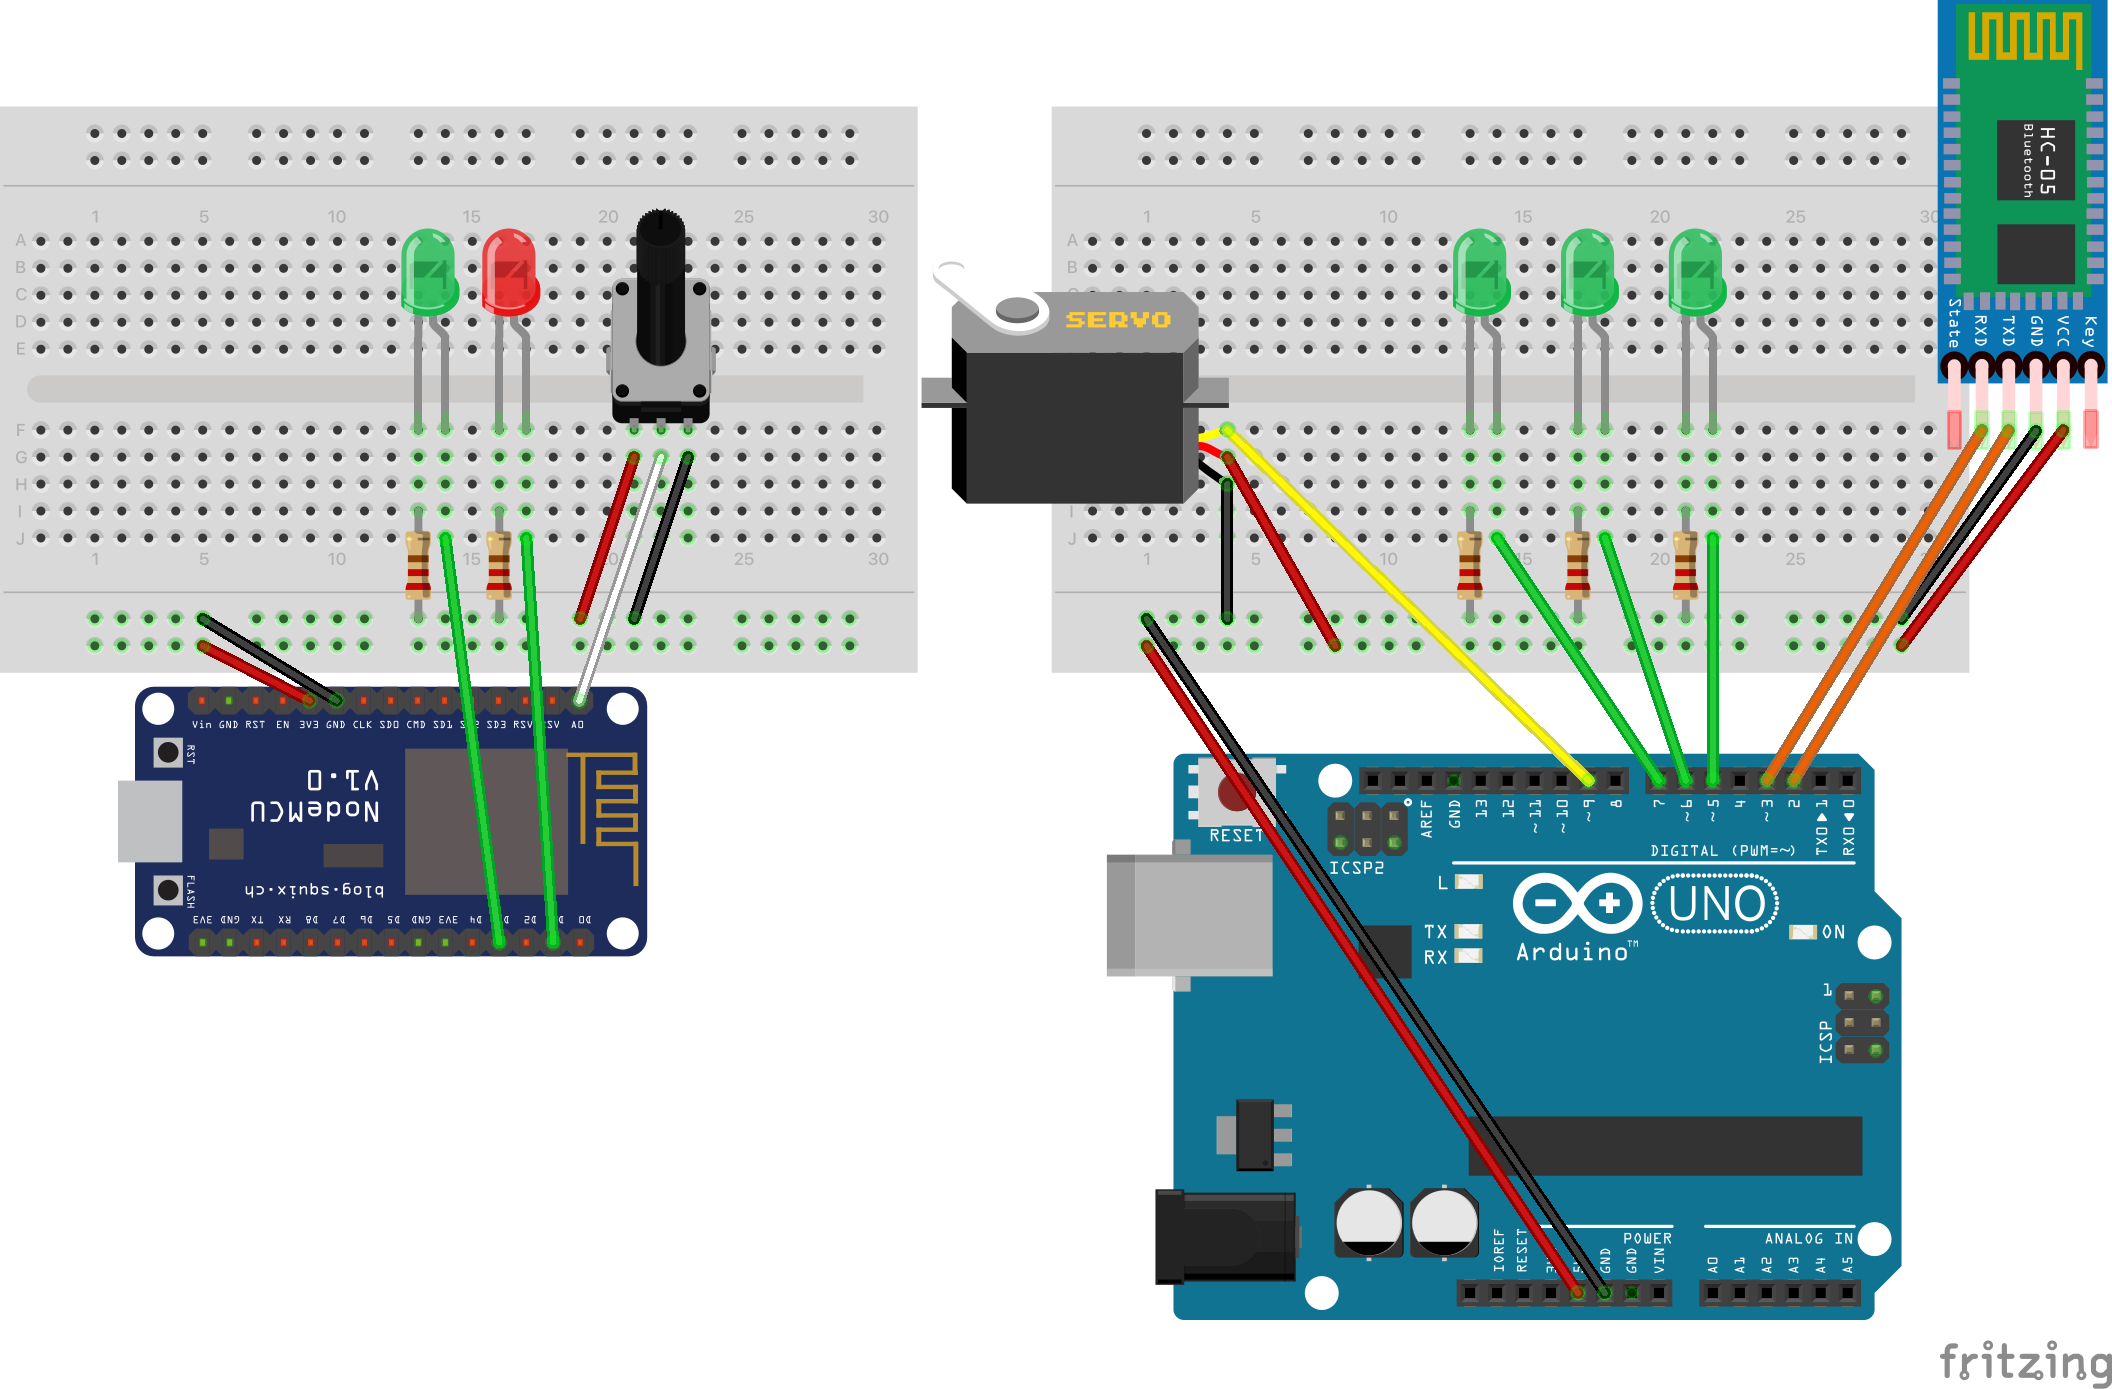
\includegraphics[width=0.9\textwidth]{"img/HardwareSchemas.png"}    
			\caption{Schemi dei circuiti per le componenti Controller ed Edge}
		\end{figure}
		\section{Design architetturale}
			\subsection{Dashboard}
			Il sito che realizza la ``Dashboard" è realizzato mediante risorse statiche dotate
			della struttura di base, ma senza alcuna informazione dentro. I dati vengono inseriti e il
			comportamento messo in atto mediante chiamate asincrone effettuate dallo \textit{user agent}
			una volta che la pagina è totalmente caricata, permettendo perciò di non avere pagine web
			dinamiche che necessitano \textit{preprocessing} lato server.
			\begin{figure}[H]
				\centering
				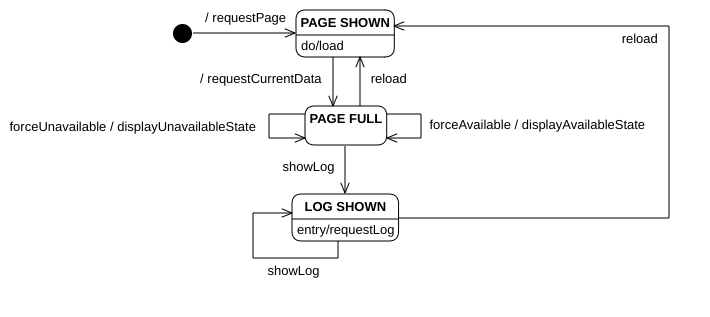
\includegraphics[width=0.7\textwidth]{"img/DashboardStatechart.png"}    
				\caption{Diagramma di stato per la componente Dashboard}
			\end{figure}
			\subsection{Controller}
			Il sistema ``Controller" è costituito da due componenti fondamentali, una di \textit{Model}
			e una di \textit{Controller}, cercando di replicare il pattern MVC senza però una componente
			di \textit{View}. Il \textit{Controller} è realizzato dal pattern ``Event-loop" dove il
			sistema resta in attesa di nuovi messaggi arrivati mediante Bluetooth e, nel momento in cui
			questi arrivano, vengono convertiti da messaggi ad eventi, cioè da elementi di Model ad
			elementi di Controller. A questo punto, si controlla se nella \textit{event queue} sono
			presenti eventi e, se così è, si estraggono e si eseguono i relativi \textit{handler}, che
			conterranno il comportamento da eseguire in caso accada quello specifico evento. I
			messaggi che può perciò ricevere Arduino sono o per iniziare il deposito per uno dei tre
			tipi di rifiuto oppure per richiedere un estensione di tempo per il deposito.
			\begin{figure}[H]
				\centering
				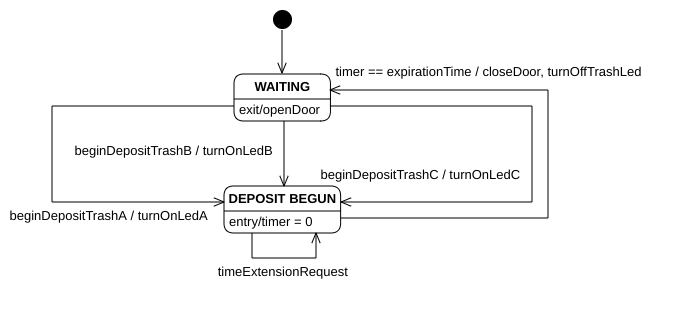
\includegraphics[width=0.7\textwidth]{"img/ControllerStatechart.png"}    
				\caption{Diagramma di stato per la componente Controller}
			\end{figure}
			\subsection{App}
			L'applicazione è costituita da una sola Activity che possiede i bottoni necessari per
			effettuare tutte le azioni necessarie all'applicazione. Questi vengono abilitati e
			disabilitati mano a mano che si passa attraverso le varie fasi del deposito di rifiuti.
			Inizialmente è infatti possibile solamente connettersi ad un bidone via Bluetooth o
			richiedere un token con i due bottoni a disposizione. Quando si è connessi e si ha anche
			ricevuto un token l'\textit{app} abilita i bottoni per scegliere il tipo di rifiuto e
			conseguentemente far partire il deposito, disabilitando i precedenti. Premuto uno qualsiasi
			dei tre bottoni questi vengono disabilitati e poi viene prima informato il Service della
			richiesta e, se tutto è andato a buon fine, si comunica la stessa cosa al Controller,
			fornendogli anche il tipo di rifiuto scelto. Se anche in questo caso non si sono verificati
			errori, il deposito può iniziare e viene perciò abilitato il pulsante per l'estensione del
			tempo di deposito. Al termine del tempo, l'app si preoccuperà di comunicare al Service la
			terminazione del deposito, verrà disabilitato il pulsante per l'estensione di tempo e si
			tornerà alla configurazione iniziale dell'app. Quest'ultima controllerà se si è ancora
			connessi via Bluetooth al Controller e, in tal caso, il corrispondente bottone verrà
			disabilitato non essendo necessario.
			\begin{figure}[H]
				\centering
				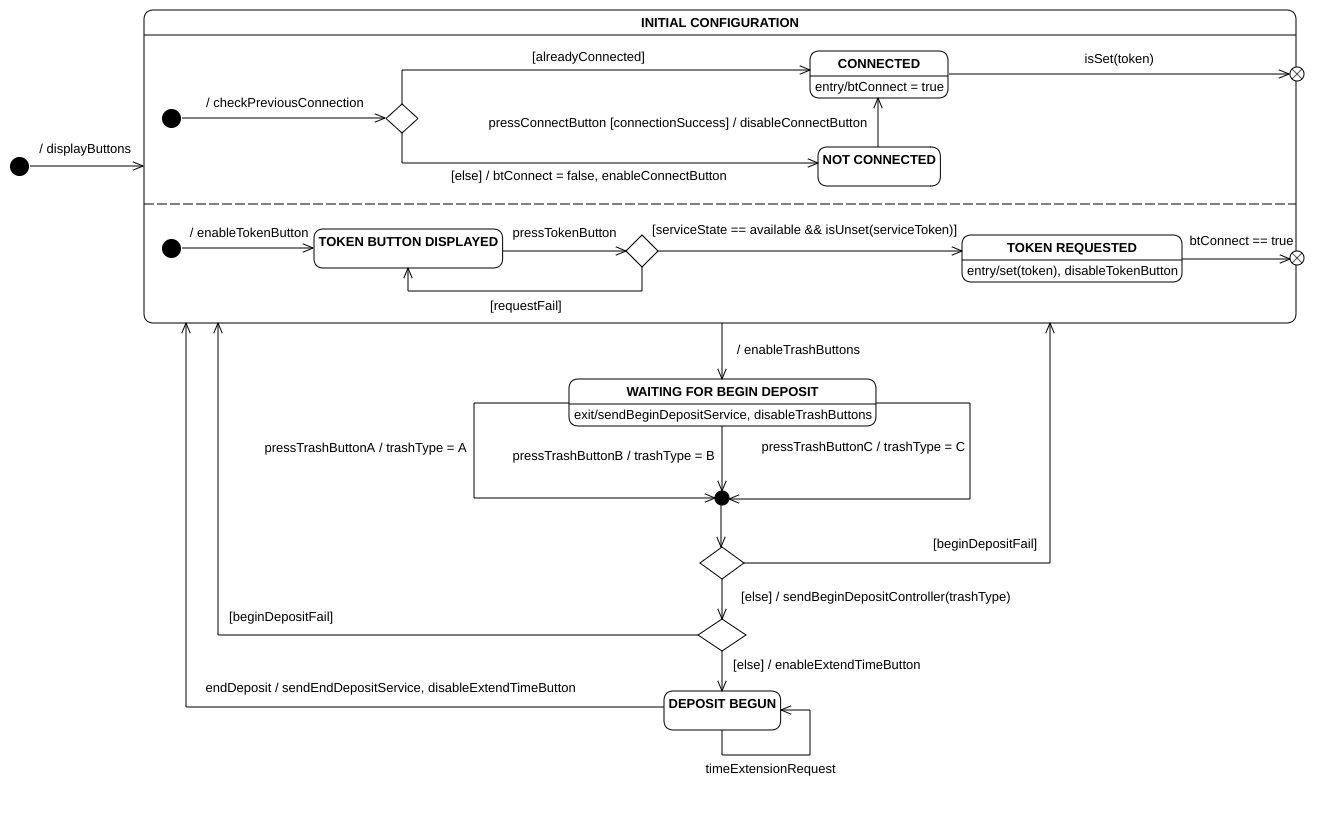
\includegraphics[width=1.03\textwidth]{"img/AppStatechart.png"}    
				\caption{Diagramma di stato per l'applicazione}
			\end{figure}
			\subsection{Edge}
			Il sistema "Edge" del sistema è anch'essa costituita da due componenti fondamentali: una di
			\textit{Model} e una di \textit{Controller}, rispecchiando una versione modificata del
			pattern MVC senza la componente di \textit{View}.\newline
			Il Controller è stato realizzato mediante il pattern ``Event-loop", dove ad ogni iterazione
			del ciclo di esecuzione principale si controlla se sono arrivati nuovi messaggi sotto forma
			di richieste HTTP al Web Server che esegue all'interno del SoC. Se sono presenti connessioni
			da parte dell'unico possibile client in attesa, il Service, queste vengono stabilite e si
			estraggono i dati da esse per formare oggetti di tipo Message. Questi vengono poi, uno per
			iterazione, trasformati dall'Event-loop in eventi ed affidati al cosiddetto ``EventHandlerManager". Questo si preoccupa di metterli in una coda di eventi che è il cuore
			del pattern ``Event-loop". Dopodiché, si estrae un evento per iterazione dalla coda e lo si
			riaffida all'EventHandlerManager perché esegua il corrispondente comportamento associato a
			quell'evento, ovverosia il suo \textit{handler}. Questo è stato fatto in tal modo affinché
			l'Event-loop sia sempre a conoscenza di quale evento sta venendo eseguito ad ogni iterazione,
			anche se questa scelta è di per sé irrilevante perché non ci sono eventi che vanno gestiti in
			maniera diversa dagli \textit{handler} che sono ad essi associati.\newline
			I possibili eventi che
			Edge riesce a gestire sono: il passaggio allo stato ``\textit{unavailable}" e quello allo
			stato ``available", dove quest'ultimo presenta la particolarità di azzerare il peso
			correntemente contenuto nel bidone perché corrisponde all'azione di svuotamento del bidone
			stesso e alla sua rimessa in funzione. Questi due cambi di stato possono essere effettuati
			in qualsiasi momento, anche durante il deposito.
			Oltre a ciò, è possibile richiedere ad Edge l'inizio
			di un deposito, cosa che verrà fatta esclusivamente se lo stato corrente è pari a
			``available", nonché la terminazione dello stesso. Un deposito potrebbe terminare anche nel
			caso l'utente che sta effettuando il deposito appoggi troppo peso rispetto a quanto ne può
			ancora contenere il bidone. In ogni caso, al termine di una procedura di deposito viene
			segnalato il peso dei rifiuti inseriti. Da ultimo, ma non per questo meno importante, è
			possibile richiedere informazioni sullo stato corrente di Edge, come il peso correntemente
			contenuto e se è nello stato ``\textit{available}" o ``unavailable".\newline
			\begin{figure}[H]
				\centering
				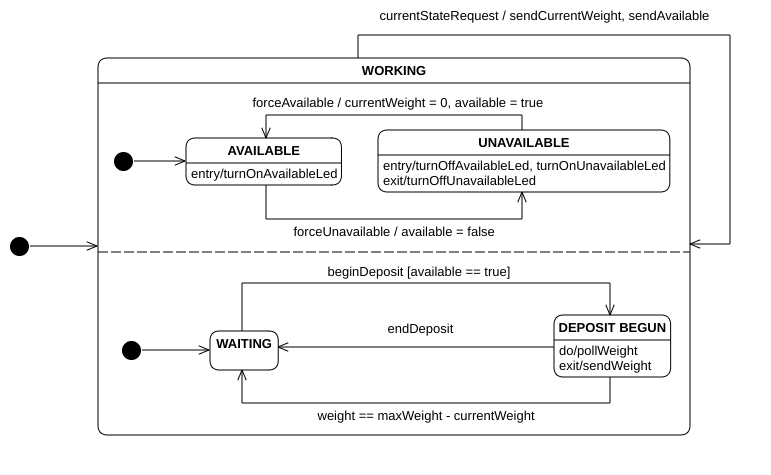
\includegraphics[width=0.8\textwidth]{"img/EdgeStatechart.png"}    
				\caption{Diagramma di stato per la componente Edge}
			\end{figure}
			\subsection{Service}
			Il sistema Service è essenzialmente il \textit{digital twin} del bidone, ovvero il suo
			doppio virtuale che permette di estrapolare informazioni da esso e fornire servizi. Poiché
			può comunicare via Internet tramite HTTP con i vari componenti del sistema, esso è composto
			sia di un web client che di un web server, nonché di una rappresentazione interna del
			componente Edge, quello dei due nel bidone con cui può direttamente comunicare. Lo
			stato di questa viene mantenuto sempre allineato con il componente fisico, così da poter
			effettuare alcune operazioni più rapidamente, senza bisogno di connettersi tutte le volte
			a quest'ultimo. Service, dialogando con la Dashboard - la quale è di fatto il suo
			\textit{frontend} -, deve poter fornire informazioni aggiornate sullo stato corrente del
			bidone - peso dei rifiuti correntemente contenuti, numero di depositi effettuati, lo stato
			vero e proprio del bidone -, ma anche il \textit{log} dei precedenti cinque giorni che
			contiene informazioni in forma riassunta sui depositi effettuati in passato. Inoltre, offre
			la possibilità di forzare lo stato ad ``\textit{available}" o ``\textit{unavailable}", che
			non fa altro che
			inoltrare la richiesta al sistema Edge e controllare successo o fallimento dell'operazione.
			\newline Dialogando con l'app, Service permette di richiedere l'inizio o la fine di un
			deposito attraverso l'uso di un token così come descritto nelle specifiche. In caso
			l'applicazione notificasse la terminazione del deposito dopo che questo è già stato terminato
			da Edge perché l'utente ha raggiunto il peso massimo consentito di rifiuti per il bidone,
			Service si premura di non notificare nuovamente la cosa ad Edge, cosa che altrimenti farebbe.
			\begin{figure}[H]
				\centering
				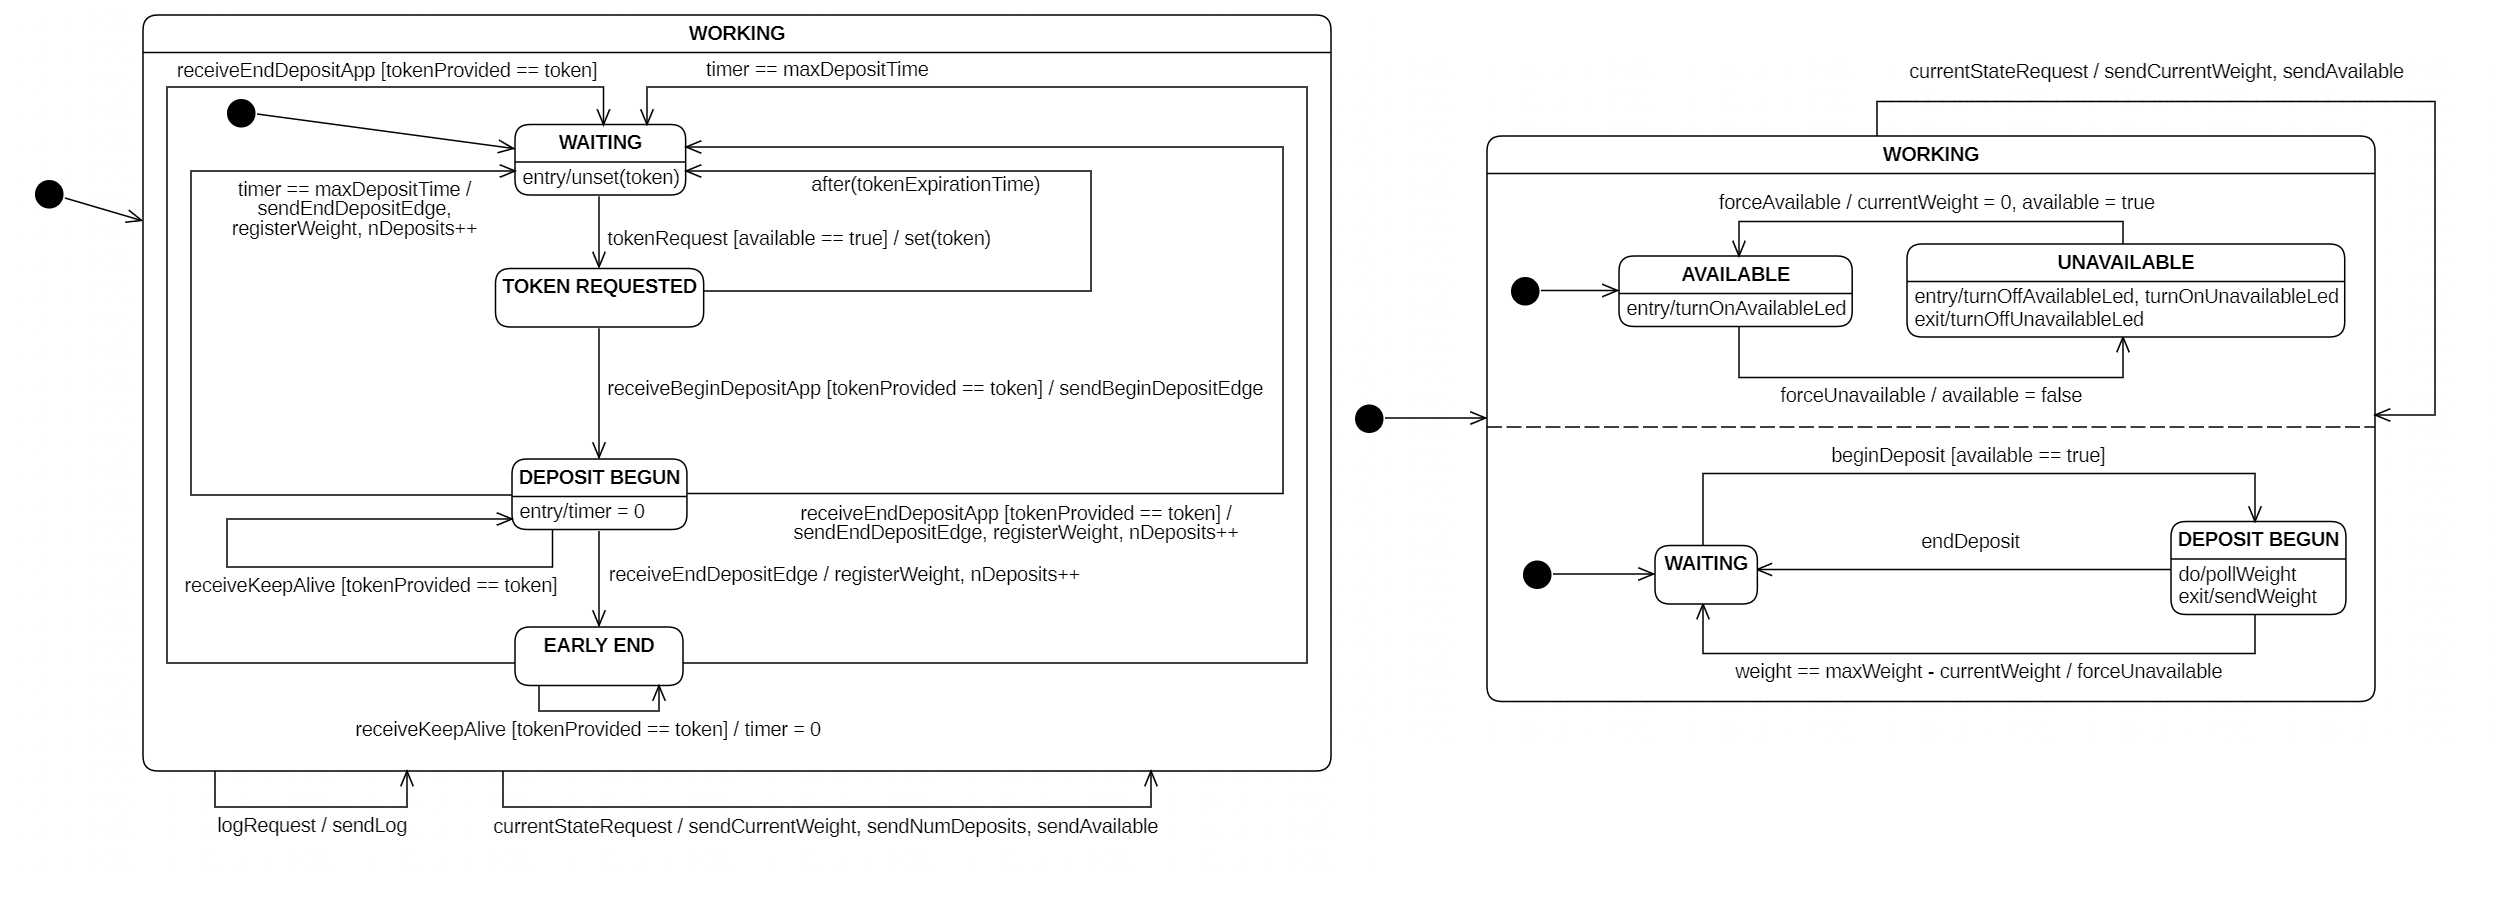
\includegraphics[width=\textwidth]{"img/ServiceStatechart.png"}    
				\caption{Diagramma di stato per la componente Service}
			\end{figure}
		\section{Design dettagliato}
			\subsection{Dashboard}
			Il sito web della ``Dashboard" è realizzato interamente in HTML, CSS e Javascript. È stata
			utilizzata anche la libreria jQuery per semplificare l'uso di Javascript. Di questa in
			particolare è stata usata l'API per l'uso di AJAX, sfruttato per effettuare richieste
			asincrone al server ``Service" per ottenere dati in formato JSON, cioè lo stato corrente,
			il peso dei rifiuti correntemente nel bidone, il numero di depositi effettuati, il log,
			oppure per permettere la realizzazione del comportamento del sistema, cioè le
			funzionalità di forzatura dello stato ``\textit{available}" o ``\textit{unavailable}".
			\subsection{Controller}
			L'utilizzo del Bluetooth è permesso dalla libreria ``SoftwareSerial" che permette di inviare
			e ricevere dati da un qualsiasi componente che scambia dati tramite connessione seriale
			asincrona come se si stesse usando la comunicazione seriale standard fornita da Arduino.
			\newline I messaggi sono costituiti da un solo carattere e perciò, avendo una struttura così
			rigida, non è necessario l'uso di terminatori di messaggio.\newline
			In caso non sia presente alcun messaggio, l'oggetto che si occupa della comunicazione via
			Bluetooth restituisce un messaggio vuoto. Questo viene poi a sua volta convertito dal
			\textit{parser} in un evento nullo, a cui non è associato nessun \textit{handler} e che
			perciò non fa accadere nulla, in applicazione del ``Null Object" pattern.
			\subsection{App}
			Per la comunicazione via Bluetooth è stato deciso di utilizzare la libreria fornitaci dal
			professore senza applicare alcuna modifica. Inoltre, si è presupposto che il \textit{pairing}
			tra i due \textit{device}, App e Controller, sia avvenuto precedentemente e perciò basta
			stabilire una connessione tra i due.
			\subsection{Edge}
			La componente Model è suddivisa in tre sotto-componenti: una che contiene le classi che
			rappresentano i componenti fisici con cui ESP va ad interagire, una per le classi che
			contengono la logica di funzionamento dell'intero sistema, secondo un pattern di tipo
			``Strategy", che altro non sono che sotto-classi dell'interfaccia ``Handler", perciò sono
			\textit{handler} di eventi specifici, e una che contiene tutte le classi per rappresentare
			all'interno di Edge la componente Service e la possibilità di scambiare messaggi con essa.
			Service perciò, potendo sia inviare che ricevere messaggi, ed essendo questi scambiati via
			HTTP, deve poter fare sia da \textit{server} che da \textit{client} HTTP. In più, un
			messaggio è sia una \textit{request} HTTP che una \textit{response} e quindi i metodi per lo
			scambio di messaggi dovranno distinguere nella creazione di oggetti di tipo ``Message" tra
			questi due tipi di messaggi HTTP. In realtà, poiché l'unico messaggio che Edge può inviare
			è quello per la terminazione di un deposito, la \textit{response} che Service fornisce per
			questo è poco significativa, perciò si è optato per ignorarla e non far gestire i
			messaggi di \textit{response} HTTP dal metodo di ricezione dei messaggi della classe Service.
			\newline La componente di Controller invece possiede una classe che fa da madre a tutte le
			altre che è ``EventScheduler", la quale si serve di ``EventHandlerManager" che trattiene la
			coda degli eventi nonché l'insieme degli \textit{handler} eseguibili e permette le operazioni
			su di queste. È infatti possibile accodare e togliere dalla coda degli eventi uno specifico
			evento, inoltre è possibile aggiungere un handler, ma non rimuoverlo perché non c'era
			necessità di offrire questa funzionalità dato che quali e quanti sono questi viene deciso
			a priori.\newline
			Per utilizzare l'astrazione della lista, anche per poterla gestire come se fosse una coda,
			anziché usare le strutture dati \textit{array} già presenti nel linguaggio si è fatto
			ricorso alla
			libreria ``LinkedList". Per il \textit{parsing} e l'\textit{encoding} dei dati in formato
			JSON ricevuti ed inviati si è fatto ricorso alla libreria ``ArduinoJSON". Per l'utilizzo di
			un \textit{client} e un \textit{server} web si è fatto ricorso alle
			librerie ``ESP8266WiFi", ``ESP8266HTTPClient" e ``ESP8266WebServer".
			\subsection{Service}
			Per realizzare l'applicazione ci si è appoggiati al \textit{framework} ``VertX" per Java
			che fornisce già tutti gli strumenti necessari per gestire un \textit{web server}, un
			\textit{web client} e per effettuare \textit{request} o formulare \textit{response} HTTP.
			È presente inoltre una classe che rappresenta una copia mantenuta allineata del sistema
			Edge di cui Service è il \textit{digital twin}. L'oggetto prodotto da questa classe viene
			interpellato per quanto riguarda le operazioni di ottenimento dello stato corrente e viene
			aggiornato in caso di forzatura dello stato dalla Dashboard o da un deposito terminato
			anticipatamente e segnalato perciò da Edge. Informazioni come il conteggio corrente dei
			depositi giornalieri nonché la quantità totale di rifiuti gettati in uno specifico bidone
			viene salvata in degli appositi file su disco, uno per giorno, che vengono poi utilizzati
			per ottenere le informazioni per costruire il \textit{log}. Non appena un'operazione ne ha
			bisogno, ma non sono presenti questi vengono creati, ma con entrambi i parametri citati
			posti a zero, così dall'operazione successiva saranno già pronti per l'uso. Per quanto
			riguarda la loro cancellazione, questa non è prevista in Service, dovrà essere l'operatore
			a cancellarli manualmente quando non saranno più necessari.
\end{document} 
